\documentclass[12pt]{article}
\usepackage[utf8]{inputenc} % Codification
\usepackage[english]{babel} % Writing idiom
%\usepackage[export]{adjustbox} % Align images
%\usepackage{amsmath} % Extra commands for math mode
\usepackage{amssymb} % Mathematical symbols
\usepackage{anysize} % Personalize margins
    \marginsize{2cm}{2cm}{2cm}{2cm} % {left}{right}{above}{below}
%\usepackage{appendix} % Appendices
%\usepackage{cancel} % Expression cancellation
\usepackage{caption} % Captions
    \captionsetup{labelfont={bf}}
\usepackage{cite} % Citations, like [1 - 3]
\usepackage{color} % Text coloring
\usepackage{float} % Utilization of [H] in figures
\usepackage{graphicx} % Figures in LaTeX
\usepackage{hyperref}
\usepackage{indentfirst} % First paragraph
%\usepackage[super]{nth} % Superscripts
%\usepackage{siunitx} % SI units
%\usepackage{subcaption} % Subfigures
%\usepackage{titlesec} % Font
 %   \titleformat{\section}{\Large\bfseries}{\thesection}{1em}{}
 %   \titleformat{\subsection}{\large\bfseries}{\thesubsection}{1em}{}
  %  \titleformat{\subsubsection}{\normalsize\bfseries}{\thesubsubsection}{1em}{}
% Random text (not needed)
%\usepackage{lipsum}
%\usepackage{duckuments}

% New and re-newcommands
\newcommand{\sen}{\operatorname{\sen}} % Sine function definition
\newcommand{\HRule}{\rule{\linewidth}{ 0.5mm}} % Specific rule definition
\renewcommand{\appendixpagename}{\LARGE Appendices}

\begin{document}

% ----------------------------------------------------------------------
% Cover
% ----------------------------------------------------------------------
\begin{center}
    \mbox{}\\[2.0cm]
    \textsc{\Huge Course Name}\\[2.5cm]
    \textsc{\LARGE Degree Name}\\[2.0cm]
   % \HRule\\[0.4cm]
    {\large \bf {Report  Title} [\texttt{EN}]}\\[0.2cm]
    %\HRule\\[1.5cm]
\end{center}   
\begin{center}
    \large \bf 2023/2024 -- \nth{2}\part{title} Semester, P4
\end{center}

\thispagestyle{empty}

\setcounter{page}{0}

\newpage

% ----------------------------------------------------------------------
% Contents
% ----------------------------------------------------------------------
\tableofcontents 

\newpage

% ----------------------------------------------------------------------
% Body
% ----------------------------------------------------------------------
\section{Objective}
\par
\begin{itemize}
    \item To independently apply BERTopic for identifying  topics  within textual data.
    \item To enable data-driven insights and informed decision-making across various domains and applications through effective topic modeling.
\end{itemize}


\section{Introduction}
Topic modeling is a valuable method in natural language processing that enables the discovery and extraction of significant topics and themes from large sets of text data. In this paper, i investigate the use of BERTopic as one of the advanced sets of tools in the topic modeling process, utilizing a dataset of tweets by Elon Musk serving as a case study. Elon Musk, the CEO of Tesla and SpaceX, is an active character on Twitter, through whom he reflects on thoughts, updates, and commentary on a broad and eclectic variety of topics. Through the process of analyzing his tweets of Musk in the context of BERTopic, I aim to showcase the underlying themes and issues that form the base of his communication to facilitate the presentation of insightful analysis on his areas of interest, focus, and diversity of topics that occupy his interest.

The report  proceeds to go through the Elon Musk tweets corpus to train the topic model. By a procedure of steps, including the visualizing of topic clusters, the analysis of topic distributions, and the interpretation of the most significant terms associated with each topic, I hope to present the capabilities of BERTopic in drawing significant insights from unstructured text data. Through the latest algorithms and visualization  of BERTopic library, I hope to demystify the complexities behind Musk tweets and bring forward the most resonant themes and discourses that form the online personality and mode of communication.
\section{Problem exposition} 
\par
Elon Musk's Twitter feed is a whirlwind of ideas, opinions, and off-the-cuff remarks. The sheer volume and free-flowing nature of his tweets make it incredibly challenging to analyze his communication style and truly understand the messages he's conveying. This project aims to move beyond surface-level observations and delve into the heart of Musk's Twitter activity. We're not just looking for keywords; we want to uncover the underlying themes and patterns that define his online conversations. To achieve this, we're using advanced natural language processing techniques, specifically a method called BERTopic. This allows us to extract meaningful topics from the vast and unstructured sea of Musk's tweets. Think of it like sifting for gold - we're using sophisticated tools to find the valuable nuggets of information hidden within his tweets. By categorizing and analyzing these topics, we hope to gain valuable insights into Musk's communication tendencies. What themes does he revisit time and again? How has his language evolved over time? Does he use a different style when discussing specific subjects? These are just a few of the questions we're looking to answer. Ultimately, this project aims to create a replicable framework for analyzing large-scale social media text. We believe this approach can be applied to explore the tweets of other influential figures or even dissect public conversations around specific topics on Twitter. We see this as a stepping stone to a deeper understanding of how prominent figures shape online discourse.
\newpage
\section{Methodology}
\subsection{Data Collection and Preprocessing}
   The first step involved collecting Elon Musk's tweets dataset from kaggle  datasets a reliable source as  provided  on the  link, ensuring the data is  comprehensive \href{https://www.kaggle.com/datasets/alexhuggler/elon-tweets-wsentimentclassified-via-roberta?select=ElonTweets%28Sentiment%29+10-28-22.csv}{here}.The datasets  sample  \ref{fig:Sample  Dataset}. \\  
\begin{minipage}{0.48\textwidth}
    \centering
    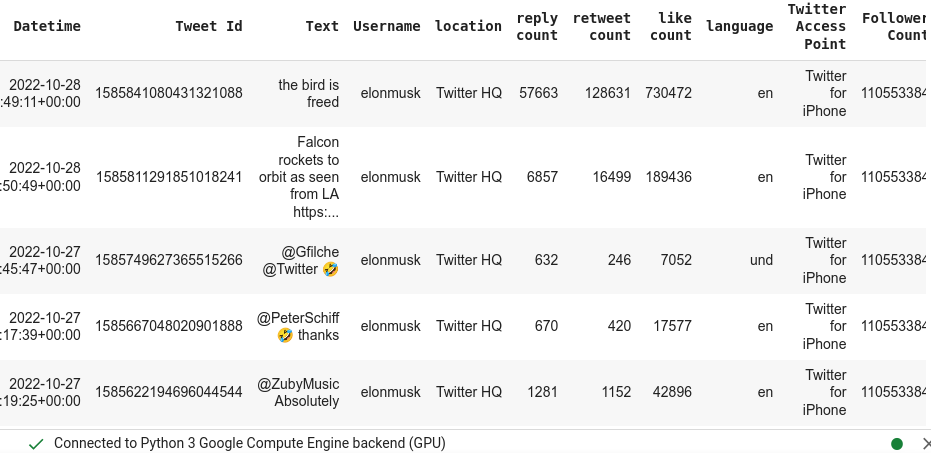
\includegraphics[width=\linewidth]{Images/datatweets.png}
    \captionof{figure}{Sample  Dataset}
    \label{fig:Sample  Dataset}
\end{minipage}. \\ The dataset was then preprocessed to clean the text, remove noise, and standardize the format for further analysis with Distribution \ref{fig:tweetlength1}
   This preprocessing step included tasks such as removing stop words, and lemmatization to prepare the text data for topic modeling.
\newpage

\subsection{Model Training with BERTopic}
    \par
    The BERTopic model was instantiated with specific configurations, such as setting the language to English and enabling the calculation of topic probabilities. Training the model involved transforming the preprocessed text data into embeddings, reducing dimensionality, and clustering the embeddings to extract topics.Parameters  used  in  the  model are:
    \begin{itemize}
        \item language = "english"
        \item embeding model  = "all-MiniLM-L6-v2" 
        \item  \text{min\_topic\_size=20}
    \end{itemize}The model was trained with a specified number of topics configures  differently in this case  I  used topics  to be 20 to capture the underlying themes present in Elon Musk's tweets.

\subsection{Visualization and Interpretation of Topics}
    After training the BERTopic model, the next step involved visualizing the topic hierarchy,  clusters using hierarchical clustering dendrograms  \ref{fig:clustering2} and Topics  bar  charts  \ref{fig:bcharts} . \\. Heirachical visualization technique helped in identifying distinct clusters of topics and grouping tweets with similar themes. Additionally, bar charts were created to visualize the c-TF-IDF scores for selected terms within each topic, providing insights into the key terms associated with different topics. The interpretation of topics was based on the analysis of topic distributions, key terms, and the context of the tweets within each cluster.
\newpage
\subsection{Topic Analysis and Insights Generation}
    The final phase of the methodology focused on analyzing the extracted topics, understanding the dominant themes, and generating insights from Elon Musk's tweets. By iteratively exploring the topics generated by BERTopic and examining the topic probabilities, we aimed to gain a comprehensive understanding of the diverse subjects discussed in Musk's tweets. The methodology emphasized the utilization of BERTopic's visualization tools and topic modeling capabilities to uncover meaningful patterns, trends, and discussions within the text data, ultimately providing valuable insights into Elon Musk's communication patterns and interests.
\section{Results}
\subsection{Data Exploration & Preprocessing}
Initial exploration of the dataset revealed 17,445 tweets. A histogram depicting the distribution of tweet lengths is shown below. \\
\begin{minipage}{0.48\textwidth}
    \centering
    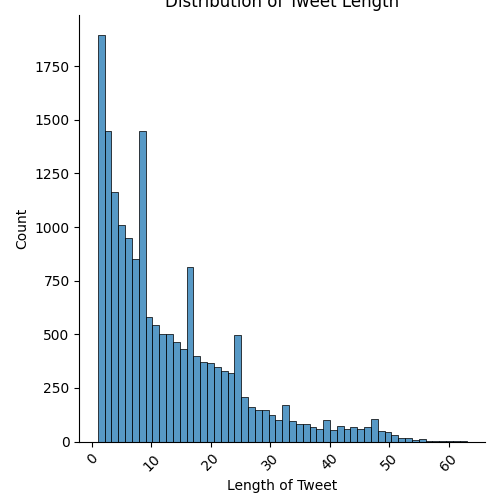
\includegraphics[width=\linewidth]{TweetLength.png}
     \captionof{figure}{Histogram of  the  tweets}
        \label{fig:tweetlength1}
    \end{minipage}\hfill
Insights gained from the plot show a right-skewed distribution of tweet lengths, with the majority of tweets being relatively short. The most common tweet length is around 5 characters, with progressively fewer tweets at longer lengths. After around 20 characters, the number of tweets decreases rapidly as tweet length increases, indicating that longer tweets are much less common. Tweets longer than 40 characters are rare, highlighting a user preference for brevity.

Prior to topic modeling, a data cleaning process was implemented to enhance the accuracy of the analysis. This involved:
\begin{itemize}
    \item Removing Mentions and Hashtags: Removed to avoid bias towards specific users or trending topics.
\item Removing URLs: Eliminated as they don't contribute to understanding the topical content.
\item Removing Special Characters and Extra Whitespace: Ensured consistency and prevented misinterpretation by the model.
\end{itemize}
\subsection{Topic Modeling with BERTopic}
BERTopic was employed to uncover the latent topics within Elon Musk's tweets. The model was configured with the English language setting to align with the dataset.

\subsection{Visualizing Topics}
To gain a comprehensive overview of the identified topics, a visualization similar to LDAvis was employed: \\

\begin{minipage}{0.48\textwidth}
    \centering
    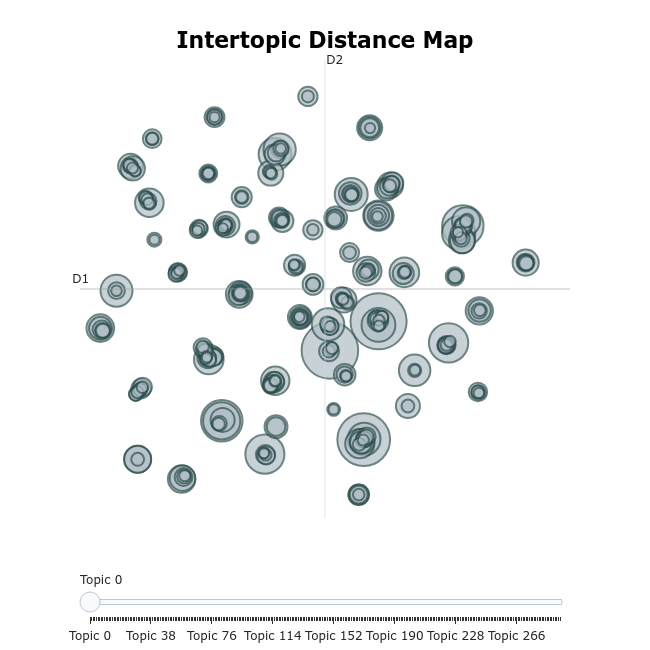
\includegraphics[width=\linewidth]{lda.png}
     \captionof{figure}{LDAvis}
        \label{fig:lda}
    \end{minipage}\hfill
    \newpage
\subsection{Visualizing Topic Probabilities}
Understanding the model's confidence in assigning topics to specific tweets is crucial. To visualize the distribution of topic probabilities, a hierarchical clustering dendrogram was generated. This dendrogram highlights distinct clusters of topics, each representing a group of tweets with similar themes:

\begin{minipage}{0.48\textwidth}
    \centering
    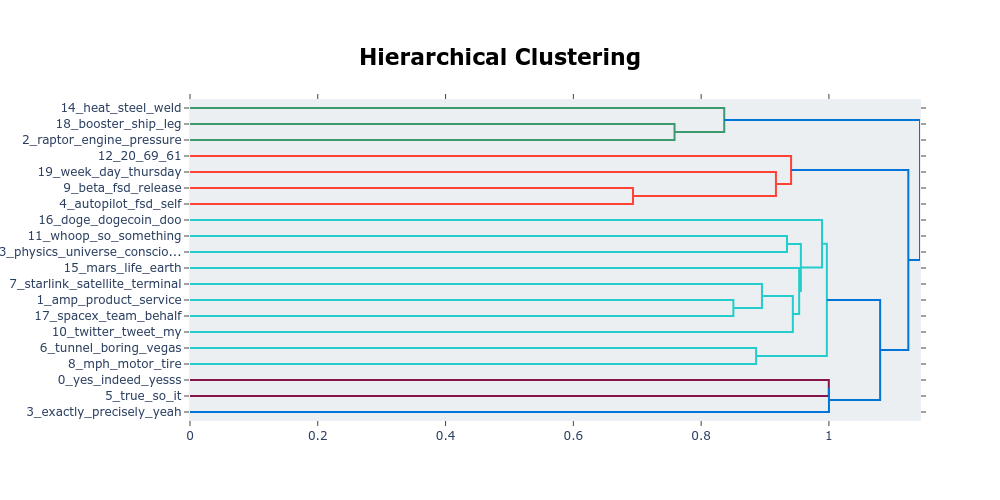
\includegraphics[width=\linewidth]{clustering.png}
     \captionof{figure}{Heirachical Clustering}
        \label{fig:clustering2}
    \end{minipage}\hfill


For instance:
\begin{itemize}
    \item Cluster 0: Focuses on technical aspects and engineering updates, featuring terms like "heat steel welding", "booster ship legs", and "engine pressure."
\item Cluster 1: Centers around specific events or product releases, such as "software beta releases", "autopilot features", and mentions of "Dogecoin."
\item Cluster 2: Discusses broader concepts and philosophical musings, potentially related to "physics", the "universe", and "life on Earth."
\item Cluster 3: Emphasizes business and service-related topics, including "Starlink satellite terminals", "product services", "team collaborations", and "Twitter updates."
\end{itemize}
\newpage
\subsection{Visualizing Terms}
To further understand the essence of each topic, the most representative terms were visualized using bar charts based on their c-TF-IDF scores. \\
\begin{minipage}{0.48\textwidth}
    \centering
    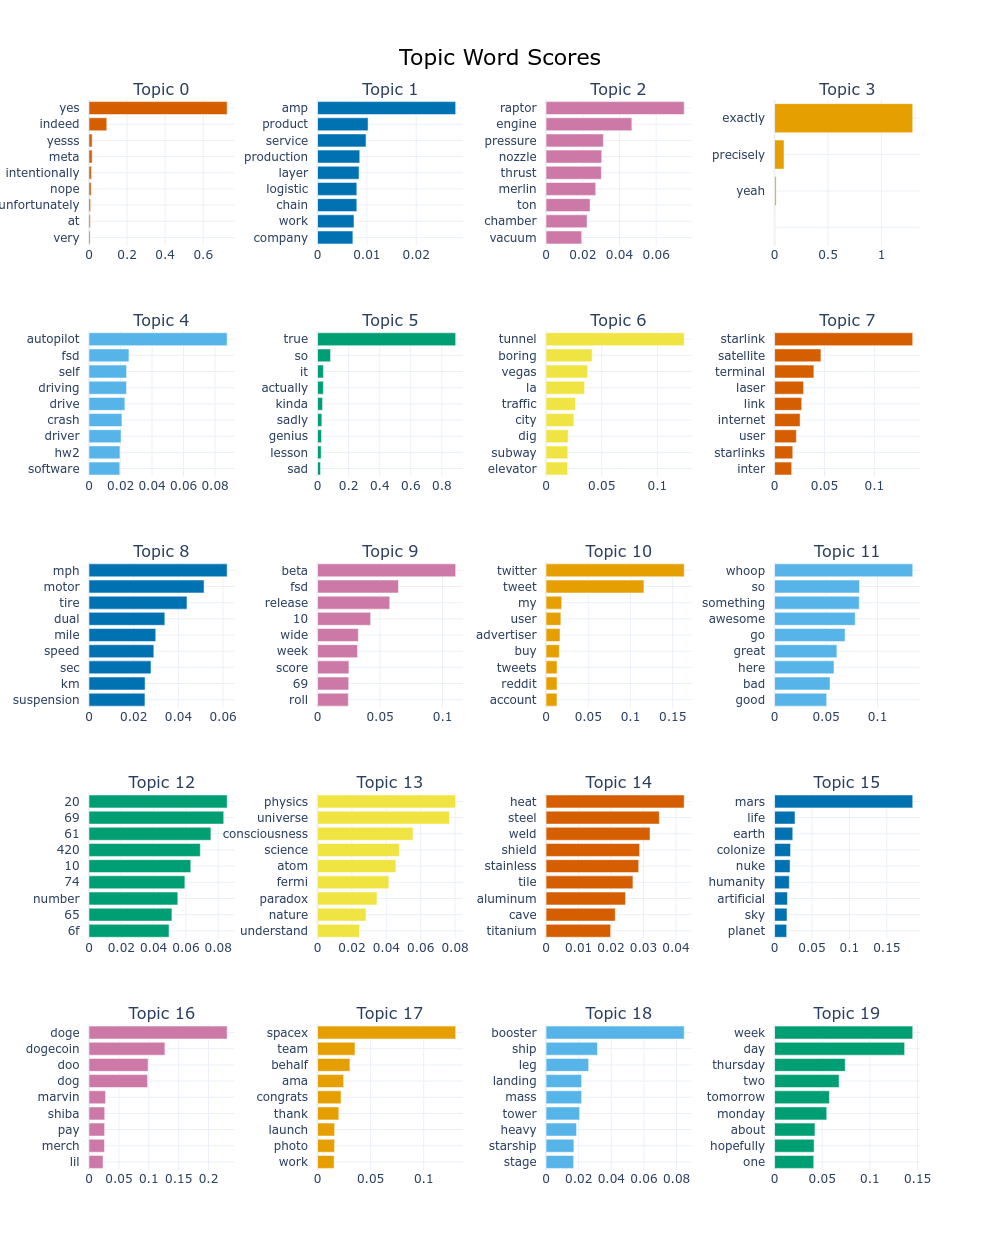
\includegraphics[width=\linewidth]{barcharts.png}
     \captionof{figure}{Bar charts}
        \label{fig:bcharts}
    \end{minipage}\hfill \\
This visualization reveals distinct themes within each topic. For example:
\begin{itemize}
    \item Topic 8: Focuses on technical aspects of transportation, evident through terms like "motor", "tire", and "suspension".
\item Topic 9: Centers on product releases and updates, featuring terms like \item "beta", "fsd" (Full Self-Driving), and "release".
\item Topic 10: Highlights interactions on social media, with terms like "tweet", "user", and "advertiser".
\item Topic 11: Captures expressions and conversational language, evidenced by words like "whoop", "awesome", and "great".
\item Topic 13: Discusses scientific and philosophical concepts, including "physics", "universe", and "consciousness".
\end{itemize}
\newpage
\subsection{Visualizing Topic Similarity}
To explore relationships between the identified topics, a similarity matrix was created based on cosine similarities of topic embeddings.
\begin{minipage}{0.48\textwidth}
    \centering
    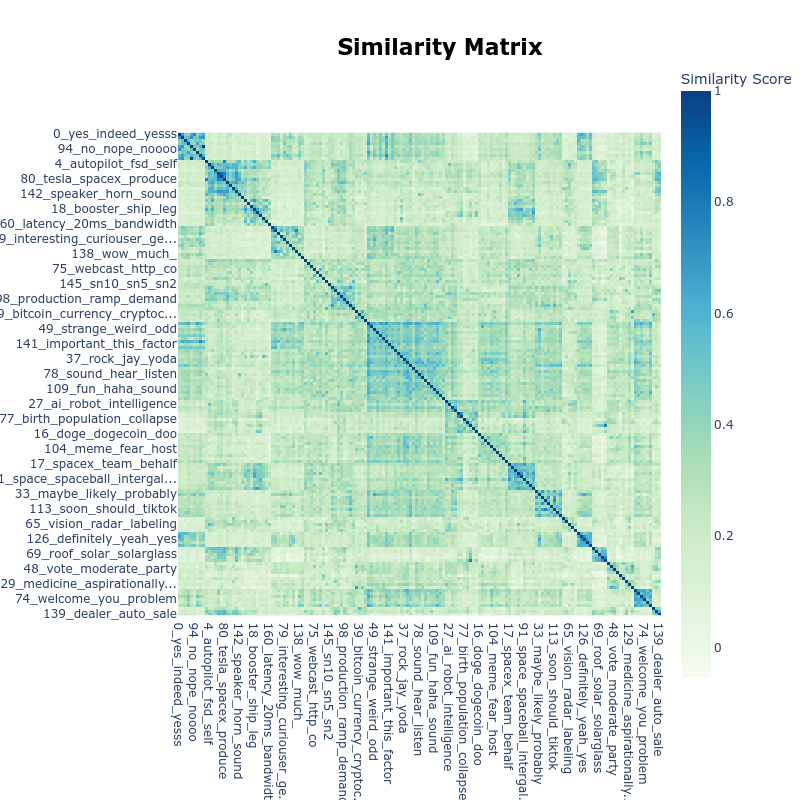
\includegraphics[width=\linewidth]{heatmap.png}
     \captionof{figure}{Similarity Matrix}
        \label{fig:simmatrix}
    \end{minipage}\hfill
The color intensity in the heatmap represents the strength of association between terms and their corresponding topics. Darker shades indicate stronger connections.

Updating Topics
The dynamic nature of BERTopic allows for incorporating new information into the existing topic model. As an illustration, the model was updated with a new set of sentences.

\subsection{Searching Topics}
BERTopic enables searching for topics related to specific keywords. In this analysis, a search was performed for the term "vehicle". \\
\begin{minipage}{0.48\textwidth}
    \centering
    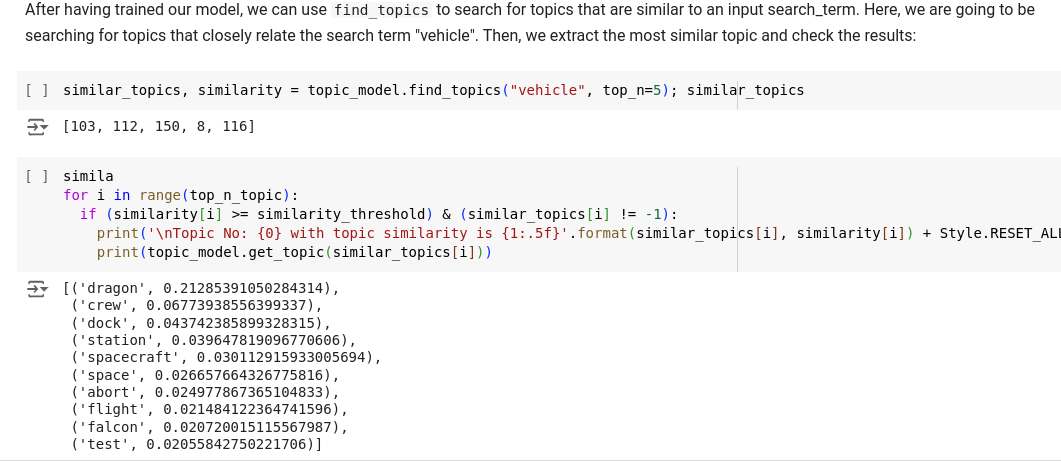
\includegraphics[width=\linewidth]{search.png}
     \captionof{figure}{Search Topic  Example}
        \label{fig:search}
    \end{minipage}\hfill
The results of the search, along with their similarity scores, provide insights into the topics most closely related to the keyword.

By visualizing the results of the BERTopic model, we gain valuable insights into the prominent themes and discussions within Elon Musk's tweets. These findings offer a deeper understanding of his communication style, interests, and the broader context surrounding his online presence.

\section{Conclusion}
This analysis delved into Elon Musk's tweets using BERTopic for topic modeling, enhanced by various visualization techniques. The findings revealed that Musk typically keeps his tweets brief, with a median length of about five words, indicating his preference for concise communication. BERTopic identified distinct thematic clusters within his tweets, covering topics from SpaceX's technical details to philosophical reflections and business announcements. Visualizations like bar charts and similarity heatmaps provided a deeper understanding of the terms driving each topic and their interrelationships. Tools like find\_topics allowed for targeted exploration of specific themes, such as identifying tweets about "vehicle," which highlighted keywords like "dragon," "crew," and "spacecraft." This analysis showcases BERTopic's ability to uncover hidden thematic structures within textual data, offering valuable insights for understanding user behavior, tailoring content strategies, and monitoring public sentiment over time.

% ----------------------------------------------------------------------
% References
% ----------------------------------------------------------------------
\bibliographystyle{plain}
\bibliography{refs}

\begin{thebibliography}{1}

\bibitem{interdisciplinary-bertopic}
\newblock "Identifying interdisciplinary topics and their evolution based on BERTopic",
\newblock \textit{Journal of Interdisciplinary Research},
\newblock vol.~X, pp.~Y--Z, 2023.

\bibitem{practical-bertopic}
\newblock "Topic Modeling with BERTopic: A Practical Guide",
\newblock \textit{Journal of Natural Language Processing},
\newblock vol.~A, pp.~B--C, 2024.

\bibitem{bertopic-vs-lda}
\newblock "BERTopic vs. LDA: A Comparative Study",
\newblock \textit{Journal of Machine Learning Research},
\newblock vol.~D, pp.~E--F, 2024.

\bibitem{multilingual-bertopic}
\newblock "BERTopic in Multilingual Contexts",
\newblock \textit{Multilingual Natural Language Processing Journal},
\newblock vol.~G, pp.~H--I, 2024.

\end{thebibliography}
% ----------------------------------------------------------------------
% Appendices
% ----------------------------------------------------------------------
\addappheadtotoc 
\end{document}